\documentclass[notes]{beamer}

\usepackage{default}
\usepackage{pgfpages}
\usepackage{pgf-pie}
\usepackage{ifthen}

\usetheme{Szeged}
\usecolortheme{dolphin}

\title{Natural Language processing for Knowledge Representation}
\subtitle{Problem statement}

\author{Jens Claes}
\date{7 november 2016}

\setbeamertemplate{note page}{\pagecolor{yellow!25}\insertnote}
\newcommand{\seperation}{
	\vspace{1em}
	\ppause
}
\newcommand{\sseperation}{
	\vspace{1em}
}
\newcommand{\hitem}{
	\ppause
	\item
}
\newcommand{\ppause}{\onslide<+>}
\newcommand{\nnote}[1]{\note<.>{#1}}
\setbeamercovered{%
	still covered={\opaqueness<1->{0}},
	again covered={\opaqueness<1->{60}}
}
\setbeameroption{hide notes} % Only slides
%\setbeameroption{show notes on second screen=right} % Both

%\graphicspath{ {../images/} }

\setbeamertemplate{bibliography item}{\insertbiblabel}
\begin{document}
	\frame{\titlepage}
	\section{Probleem}
	\begin{frame}{Situatie I}
		\begin{itemize}
			\hitem Specificaties in natuurlijke taal
			\item Door domein expert
			
			\seperation
			
			\item Vertaald naar programma's
			\item Inconsistent, moeilijk aanpasbaar
			
			\seperation
			
			\item Antwoord: Knowledge base paradigma
		\end{itemize}
		
		\note<1>{Businesses = ruled by requirements / specifications}
		\note<2>{Vroeger: omzetten naar verschillende programma's: incosistenties + moeilijk aanpasbaar, ...}
		\note<3>{KBS paradigma lost deze problemen op... maar creëert er nieuwe}
	\end{frame}
	\begin{frame}{Situatie II: KBS paradigma}
			\begin{itemize}
				\hitem Requirements in natuurlijke taal
				\item Door domein expert
				\nnote{KBS: nog steeds in natuurlijke taal. Niet meer per se alles al vastgelegd als een specificatie}
				
				\seperation
				
				\item Vertaald naar formele taal
				\item Door KBS expert
				\nnote{Iemand anders doet vertaling. Tweede specificatie + extra werk}
				
				\seperation
				
				\item Domein expert: geen formele taal
				\item KBS expert: geen domeinkennis
				\item $\Rightarrow$ Feedback loop beperkt
				\nnote{KBS kent domein niet en domain expert kent logica niet: moeilijk om feedback te geven over tweede vertaling}
				
				\seperation
				
				\item Kunnen we een formele taal ontwerpen die toegankelijk is voor domein experts, rijk genoeg is voor praktische problemen en toepasbaar is binnen KBS
				\nnote{Probleemstelling thesis}
				
				\seperation
				
				\item Antwoord: Formele \textbf{natuurlijke} talen?
				\nnote{Een formele taal nodig die toegankelijk is voor domain expert. Op zijn minst om feedback te kunnen geven over de vertaling, op zijn best om de KBS expert uit het plaatje te verwijderen}
			\end{itemize}
	\end{frame}
	
	\begin{frame}{Waarom}
		\begin{itemize}
			\hitem Natuurlijke taal al gebruikt. 
			\item Stel (ook) formele specificatie erin op.
			\begin{figure}
				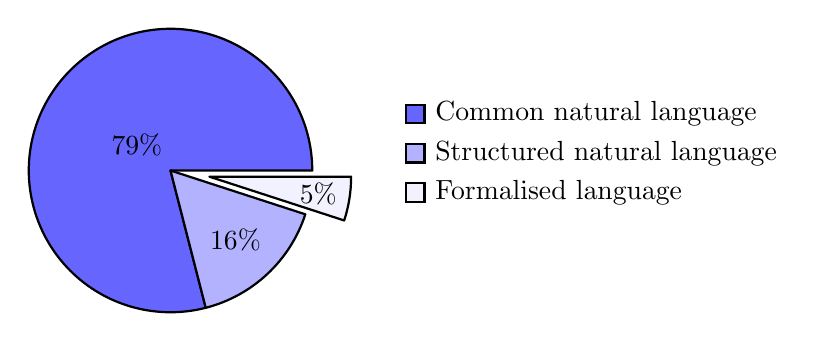
\begin{tikzpicture}
				    \pie[text = legend, radius = 1.8, explode = {0, 0, 0.5}, color = {blue!60, blue!30, blue!5}]{79/Common natural language, 16/Structured natural language, 5/Formalised language}
				\end{tikzpicture}
				\caption{Use of language in Requirements Engineering in 1999 (From figure 5 in \cite{Luisa2004})}
			\end{figure}
			
			\hitem Leesbaar voor domein expert, KBS expert en machines
		\end{itemize}
		
		\note<1>{
			\begin{itemize}
				\item Domein experts stellen de specificatie op. Zij kennen geen formele talen.
				\item Controlled natural language is wel mogelijk. Soms wordt het al gebruikt. Meestal minder formele talen dan. Enkel voor de leesbaarheid.
			\end{itemize}
		}
		\note<2>{Machines kunnen specificaties lezen en omzetten als input voor KBS}
	\end{frame}
	
	\section{Doel}
	\begin{frame}{Doel Thesis}
		\begin{itemize}
			\hitem Nieuwe taal construeren
			\item Basis FO concepten
			\item Toegankelijk voor domein experten
			
			\seperation
			\item Kunnen we $FO(.)^{IDP3}$ \cite{Bruynooghe2014} constructs toevoegen?
			\item Kunnen we een NLP interface aanbieden voor IDP?
			
			\seperation
			\item Kunnen we dynamische systemen toevoegen?
		\end{itemize}
		\note<1>{Nieuwe formele natuurlijke taal met een simpele BNF zodat lookahead mogelijk is, indien later nog gewenst: Makkelijker te leren + tools rond te bouwen}
		\note<2>{
			\begin{itemize}
				\item Arithmetic toevoegen? (al deels in ACE)
				\item Aggregates toevoegen?
				\item Types toevoegen?
				\item Partial functions toevoegen?
				\item Inductive definitions toevoegen?
				\item NLP vragen als entrypoint voor verschillende inferenties?
				\item Kunnen we vocabulary en structures voorstellen? Of er automatisch uithalen?
			\end{itemize}
			$\Rightarrow$ Hoe volledig kunnen we de interface naar IDP maken?
		}
		\note<3>{Extra: Kunnen we dynamische systemen modelleren met natuurlijke taal (gebruik makend van Event-based ipv LTC).}
	\end{frame}
		
	\section{Voorbeeld}
	\begin{frame}{Voorbeeld}
		\begin{itemize}
			\hitem Only employees younger than 18 or at least 60 years or employees with at least 30 years of service will receive 5 extra days \cite{VacationDays}
			\note<.>{Een voorbeeld van Jan Vanthienen.}
			
			\seperation
			
			\item If the age of the employee is less than 18 or greather than 60 then he receives 5 extra days
			\item If the years of service of the empolyee is a least 30 then he receives 5 extra days
			\note<.>{Een mogelijke vertaling naar een meer formele taal.}
			
			\seperation
			
			\item $\forall$ emp: receives\_extra\_days(emp, 5)
				$\leftarrow age(emp) < 18 \vee age(emp) > 60$.
			\item $\forall$ emp: receives\_extra\_days(emp, 5)
				$\leftarrow years\_of\_service(emp) >= 30.$
			\note<.>{Een mogelijke vertaling naar FO(.)}
		\end{itemize}
	\end{frame}

	\section{Eerder werk}
	\begin{frame}{Eerder werk}
		\begin{itemize}
			\ppause
			\hitem Circe \cite{Ambriola1997}
			
			\seperation
			\item Attempto Controlled English (ACE) \cite{Fuchs2008}
			
			\seperation
			\item Processable ENGlish (PENG) \cite{Schwitter2003, Schwitter2006}
			\item PENG Light \cite{Schwitter2008}
			
			\seperation
			\item Model checking \cite{Flake2002, Konrad2005}
		\end{itemize}
		
		\note<1>{
			Al vele CNL's gemaakt, niet allemaal even formeel. Sommige enkel als minder amibuge taal: RuleSpeak, RuleCNL, CELT (ontologie wordt gebruikt om te parsen), ... Zie Kuhn et al (2014) \cite{Kuhn2014} voor een overzicht + classificatie
		}
		\note<2>{
			Circe
			\begin{itemize}
				\item Framework
				\item Requirements Engineering: Glossary + Requirements
				\item Domein-specifieke regels. E.g. Data flow regels
				\item MAS: Model, Action, Substution rules
				\item automatische checks voor specificatie (e.g. input ontbreekt in data flow) + automatische diagrammen
				\item Verschillende domeinen geïmplementeerd: data flow, entity relationship, ...
			\end{itemize}
			\textbf{Doel is om niet domein-specifiek te gaan!}
		}
		\note<3>{
			ACE
			\begin{itemize}
				\item formele, natuurlijke taal. Simpele en composiet zinnen, vragen en commando's
				\item subset van FO ondersteund (niet geheel duidelijk wat wel en wat niet, formele taal maar heel vrij).
				\item Anaforische referenties heel goed (a (blue) car $\leftarrow$ the (blue) car. She $\leftarrow$ herself, ...): Discourse Representation Theory
				\item Vooral veel onderzoek voor semantische web, ook 1 master thesis rond semantisch KBS systeem
				\item Multi-words minder ondersteund: interested-in vs interested in
				\item Soms ambigu in Engels maar niet in ACE. Paraphrasing om ambiguïteit te verminderen.
				\item Ongeveer 2 dagen om de basis te leren\cite{Fuchs2008}
				\item Meerdere tools: APE (parser), RACE (reasoner), ACE Wiki (OWL wiki)
				\item Moeilijk uit te breiden. Meeste research over hoe men ACE kan gebruiken in andere domeinen
			\end{itemize}
			\textbf{Doel: Simpelere taal maken. Anaforische referentie is al volledig onderzocht, dus eventueel enkel in simpele vorm overnemen. Vooral ook FO(.) concepten toevoegen.}
		}
		\note<4>{
			\begin{itemize}
				\item PENG
				\begin{itemize}
					\item OWL DL: Description Logics, geen FO
					\item Taal moet niet geleerd worden door look ahead tool
				\end{itemize}
				\item PENG Light
				\begin{itemize}
					\item Nieuwe versie van PENG
					\item Description Logics en nu ook FO
					\item Lookahead, bidirectional: vragen met antwoord in NL
					\item Lexicon bevat logica templates
					\item Anaforische referenties (via DRT)
				\end{itemize}
			\end{itemize}
			\textbf{Doel: FO(.) concepten toevoegen, lexicon zonder templates, vragen beantwoorden maar dan voor FO(.)}
		}
		\note<5>{
			Dynamische systemen: Model checking bestaat al. Systemen zelf nog niet.
			\begin{itemize}
				\item Konrad et al (2005) \cite{Konrad2005}
				\begin{itemize}
					\item Eindige subset
					\item Vertaald naar meerdere talen
					\item Metric Temporal Logic (MTL), Timed CTL (TCTL), Real-time graphical interval logic (RTGIL).
				\end{itemize}
				\item Flake et al (2002) \cite{Flake2002}
				\begin{itemize}
					\item Naar Clocked CTL
					\item "Simpele" 1-op-1 mapping
					\item $\Rightarrow$ Simpele BNF: makkelijke look-ahead mogelijk
				\end{itemize}
			\end{itemize}
			\textbf{Doel: ook dynamische systemen zelf ondersteunen, niet enkel de model checking}
		}
	\end{frame}
			
	\section{Referenties}
	\begin{frame}[allowframebreaks]{Referenties}
		\bibliographystyle{plain}
		\bibliography{probleemstelling}
	\end{frame}
	
\end{document}
